\documentclass{extbook}[14pt]
\usepackage{multicol, enumerate, enumitem, hyperref, color, soul, setspace, parskip, fancyhdr, amssymb, amsthm, amsmath, latexsym, units, mathtools}
\everymath{\displaystyle}
\usepackage[headsep=0.5cm,headheight=0cm, left=1 in,right= 1 in,top= 1 in,bottom= 1 in]{geometry}
\usepackage{dashrule}  % Package to use the command below to create lines between items
\newcommand{\litem}[1]{\item #1

\rule{\textwidth}{0.4pt}}
\pagestyle{fancy}
\lhead{}
\chead{Answer Key for Makeup Progress Quiz 3 Version B}
\rhead{}
\lfoot{1648-1753}
\cfoot{}
\rfoot{Summer C 2021}
\begin{document}
\textbf{This key should allow you to understand why you choose the option you did (beyond just getting a question right or wrong). \href{https://xronos.clas.ufl.edu/mac1105spring2020/courseDescriptionAndMisc/Exams/LearningFromResults}{More instructions on how to use this key can be found here}.}

\textbf{If you have a suggestion to make the keys better, \href{https://forms.gle/CZkbZmPbC9XALEE88}{please fill out the short survey here}.}

\textit{Note: This key is auto-generated and may contain issues and/or errors. The keys are reviewed after each exam to ensure grading is done accurately. If there are issues (like duplicate options), they are noted in the offline gradebook. The keys are a work-in-progress to give students as many resources to improve as possible.}

\rule{\textwidth}{0.4pt}

\begin{enumerate}\litem{
Construct the lowest-degree polynomial given the zeros below. Then, choose the intervals that contain the coefficients of the polynomial in the form $x^3+bx^2+cx+d$.
\[ 5 - 3 i \text{ and } 2 \]The solution is \( x^{3} -12 x^{2} +54 x -68 \), which is option C.\begin{enumerate}[label=\Alph*.]
\item \( b \in [-9, 6], c \in [0, 6], \text{ and } d \in [-9, 1] \)

$x^{3} + x^{2} +x -6$, which corresponds to multiplying out $(x + 3)(x -2)$.
\item \( b \in [10, 13], c \in [52, 62], \text{ and } d \in [68, 76] \)

$x^{3} +12 x^{2} +54 x + 68$, which corresponds to multiplying out $(x-(5 - 3 i))(x-(5 + 3 i))(x + 2)$.
\item \( b \in [-14, -11], c \in [52, 62], \text{ and } d \in [-76, -62] \)

* $x^{3} -12 x^{2} +54 x -68$, which is the correct option.
\item \( b \in [-9, 6], c \in [-13, -1], \text{ and } d \in [4, 16] \)

$x^{3} + x^{2} -7 x + 10$, which corresponds to multiplying out $(x -5)(x -2)$.
\item \( \text{None of the above.} \)

This corresponds to making an unanticipated error or not understanding how to use nonreal complex numbers to create the lowest-degree polynomial. If you chose this and are not sure what you did wrong, please contact the coordinator for help.
\end{enumerate}

\textbf{General Comment:} Remember that the conjugate of $a+bi$ is $a-bi$. Since these zeros always come in pairs, we need to multiply out $(x-(5 - 3 i))(x-(5 + 3 i))(x-(2))$.
}
\litem{
Describe the end behavior of the polynomial below.
\[ f(x) = 8(x + 3)^{3}(x - 3)^{8}(x - 2)^{3}(x + 2)^{4} \]The solution is the graph below, which is option C.
    \begin{center}
        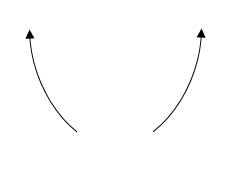
\includegraphics[width=0.3\textwidth]{../Figures/polyEndBehaviorCB.png}
    \end{center}\begin{enumerate}[label=\Alph*.]
\begin{multicols}{2}
\item 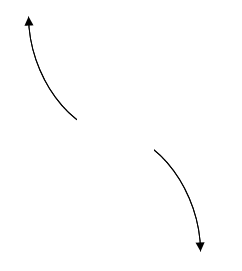
\includegraphics[width = 0.3\textwidth]{../Figures/polyEndBehaviorAB.png}
\item 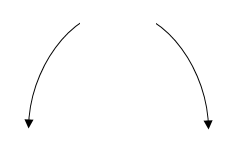
\includegraphics[width = 0.3\textwidth]{../Figures/polyEndBehaviorBB.png}
\item 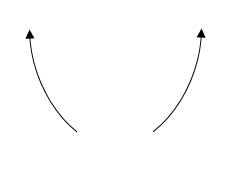
\includegraphics[width = 0.3\textwidth]{../Figures/polyEndBehaviorCB.png}
\item 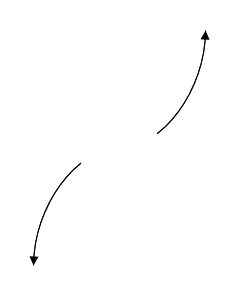
\includegraphics[width = 0.3\textwidth]{../Figures/polyEndBehaviorDB.png}
\end{multicols}\item None of the above.\end{enumerate}
\textbf{General Comment:} Remember that end behavior is determined by the leading coefficient AND whether the \textbf{sum} of the multiplicities is positive or negative.
}
\litem{
Describe the end behavior of the polynomial below.
\[ f(x) = 7(x - 4)^{4}(x + 4)^{5}(x + 3)^{3}(x - 3)^{5} \]The solution is the graph below, which is option D.
    \begin{center}
        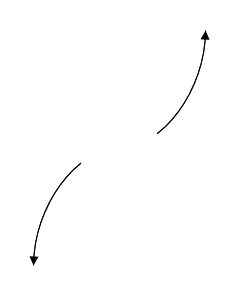
\includegraphics[width=0.3\textwidth]{../Figures/polyEndBehaviorCopyDB.png}
    \end{center}\begin{enumerate}[label=\Alph*.]
\begin{multicols}{2}
\item 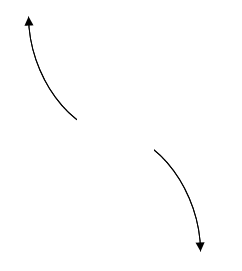
\includegraphics[width = 0.3\textwidth]{../Figures/polyEndBehaviorCopyAB.png}
\item 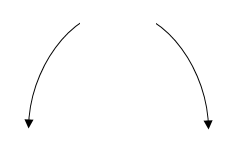
\includegraphics[width = 0.3\textwidth]{../Figures/polyEndBehaviorCopyBB.png}
\item 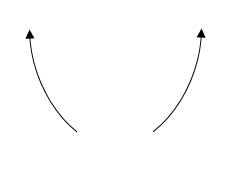
\includegraphics[width = 0.3\textwidth]{../Figures/polyEndBehaviorCopyCB.png}
\item 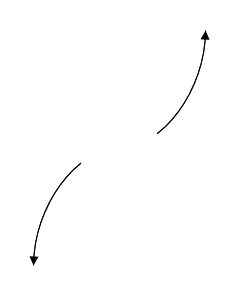
\includegraphics[width = 0.3\textwidth]{../Figures/polyEndBehaviorCopyDB.png}
\end{multicols}\item None of the above.\end{enumerate}
\textbf{General Comment:} Remember that end behavior is determined by the leading coefficient AND whether the \textbf{sum} of the multiplicities is positive or negative.
}
\litem{
Construct the lowest-degree polynomial given the zeros below. Then, choose the intervals that contain the coefficients of the polynomial in the form $ax^3+bx^2+cx+d$.
\[ 7, \frac{-1}{5}, \text{ and } \frac{2}{3} \]The solution is \( 15x^{3} -112 x^{2} +47 x + 14 \), which is option C.\begin{enumerate}[label=\Alph*.]
\item \( a \in [15, 17], b \in [110.6, 112.3], c \in [44, 57], \text{ and } d \in [-17, -12] \)

$15x^{3} +112 x^{2} +47 x -14$, which corresponds to multiplying out $(x + 7)(5x -1)(3x + 2)$.
\item \( a \in [15, 17], b \in [91.8, 95.9], c \in [-92, -82], \text{ and } d \in [14, 19] \)

$15x^{3} +92 x^{2} -89 x + 14$, which corresponds to multiplying out $(x + 7)(5x -1)(3x -2)$.
\item \( a \in [15, 17], b \in [-112.5, -108.4], c \in [44, 57], \text{ and } d \in [14, 19] \)

* $15x^{3} -112 x^{2} +47 x + 14$, which is the correct option.
\item \( a \in [15, 17], b \in [96, 100.8], c \in [-52, -44], \text{ and } d \in [-17, -12] \)

$15x^{3} +98 x^{2} -51 x -14$, which corresponds to multiplying out $(x + 7)(5x + 1)(3x -2)$.
\item \( a \in [15, 17], b \in [-112.5, -108.4], c \in [44, 57], \text{ and } d \in [-17, -12] \)

$15x^{3} -112 x^{2} +47 x -14$, which corresponds to multiplying everything correctly except the constant term.
\end{enumerate}

\textbf{General Comment:} To construct the lowest-degree polynomial, you want to multiply out $(x -7)(5x + 1)(3x -2)$
}
\litem{
Describe the zero behavior of the zero $x = 2$ of the polynomial below.
\[ f(x) = -3(x + 2)^{4}(x - 2)^{5}(x - 7)^{5}(x + 7)^{7} \]The solution is the graph below, which is option D.
    \begin{center}
        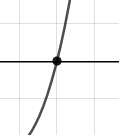
\includegraphics[width=0.3\textwidth]{../Figures/polyZeroBehaviorDB.png}
    \end{center}\begin{enumerate}[label=\Alph*.]
\begin{multicols}{2}
\item 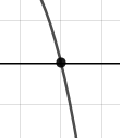
\includegraphics[width = 0.3\textwidth]{../Figures/polyZeroBehaviorAB.png}
\item 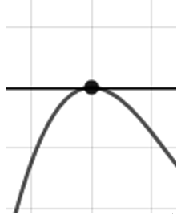
\includegraphics[width = 0.3\textwidth]{../Figures/polyZeroBehaviorBB.png}
\item 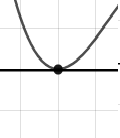
\includegraphics[width = 0.3\textwidth]{../Figures/polyZeroBehaviorCB.png}
\item 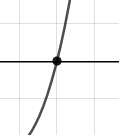
\includegraphics[width = 0.3\textwidth]{../Figures/polyZeroBehaviorDB.png}
\end{multicols}\item None of the above.\end{enumerate}
\textbf{General Comment:} You will need to sketch the entire graph, then zoom in on the zero the question asks about.
}
\litem{
Which of the following equations \textit{could} be of the graph presented below?

\begin{center}
    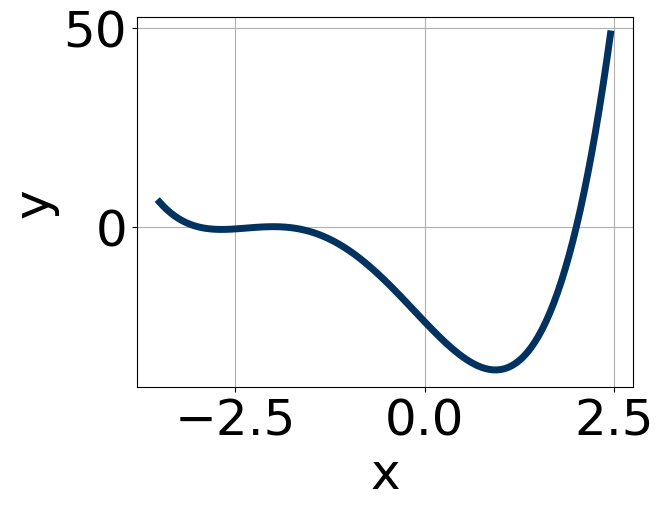
\includegraphics[width=0.5\textwidth]{../Figures/polyGraphToFunctionB.png}
\end{center}


The solution is \( -10(x - 2)^{5} (x + 4)^{7} (x + 1)^{11} \), which is option E.\begin{enumerate}[label=\Alph*.]
\item \( -8(x - 2)^{10} (x + 4)^{6} (x + 1)^{5} \)

The factors $2$ and $-4$ have have been odd power.
\item \( 12(x - 2)^{8} (x + 4)^{7} (x + 1)^{7} \)

The factor $(x - 2)$ should have an odd power and the leading coefficient should be the opposite sign.
\item \( -4(x - 2)^{10} (x + 4)^{11} (x + 1)^{11} \)

The factor $2$ should have been an odd power.
\item \( 11(x - 2)^{7} (x + 4)^{9} (x + 1)^{9} \)

This corresponds to the leading coefficient being the opposite value than it should be.
\item \( -10(x - 2)^{5} (x + 4)^{7} (x + 1)^{11} \)

* This is the correct option.
\end{enumerate}

\textbf{General Comment:} General Comments: Draw the x-axis to determine which zeros are touching (and so have even multiplicity) or cross (and have odd multiplicity).
}
\litem{
Construct the lowest-degree polynomial given the zeros below. Then, choose the intervals that contain the coefficients of the polynomial in the form $x^3+bx^2+cx+d$.
\[ 4 + 5 i \text{ and } 1 \]The solution is \( x^{3} -9 x^{2} +49 x -41 \), which is option A.\begin{enumerate}[label=\Alph*.]
\item \( b \in [-11, -5], c \in [48.79, 49.11], \text{ and } d \in [-41.09, -39.64] \)

* $x^{3} -9 x^{2} +49 x -41$, which is the correct option.
\item \( b \in [1, 6], c \in [-5.16, -3.28], \text{ and } d \in [2.13, 4.62] \)

$x^{3} + x^{2} -5 x + 4$, which corresponds to multiplying out $(x -4)(x -1)$.
\item \( b \in [1, 6], c \in [-6.36, -5.54], \text{ and } d \in [4.44, 5.18] \)

$x^{3} + x^{2} -6 x + 5$, which corresponds to multiplying out $(x -5)(x -1)$.
\item \( b \in [3, 14], c \in [48.79, 49.11], \text{ and } d \in [39.48, 43] \)

$x^{3} +9 x^{2} +49 x + 41$, which corresponds to multiplying out $(x-(4 + 5 i))(x-(4 - 5 i))(x + 1)$.
\item \( \text{None of the above.} \)

This corresponds to making an unanticipated error or not understanding how to use nonreal complex numbers to create the lowest-degree polynomial. If you chose this and are not sure what you did wrong, please contact the coordinator for help.
\end{enumerate}

\textbf{General Comment:} Remember that the conjugate of $a+bi$ is $a-bi$. Since these zeros always come in pairs, we need to multiply out $(x-(4 + 5 i))(x-(4 - 5 i))(x-(1))$.
}
\litem{
Describe the zero behavior of the zero $x = -7$ of the polynomial below.
\[ f(x) = -9(x - 4)^{5}(x + 4)^{2}(x + 7)^{11}(x - 7)^{8} \]The solution is the graph below, which is option D.
    \begin{center}
        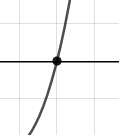
\includegraphics[width=0.3\textwidth]{../Figures/polyZeroBehaviorCopyDB.png}
    \end{center}\begin{enumerate}[label=\Alph*.]
\begin{multicols}{2}
\item 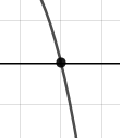
\includegraphics[width = 0.3\textwidth]{../Figures/polyZeroBehaviorCopyAB.png}
\item 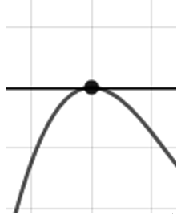
\includegraphics[width = 0.3\textwidth]{../Figures/polyZeroBehaviorCopyBB.png}
\item 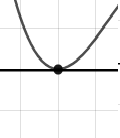
\includegraphics[width = 0.3\textwidth]{../Figures/polyZeroBehaviorCopyCB.png}
\item 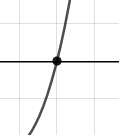
\includegraphics[width = 0.3\textwidth]{../Figures/polyZeroBehaviorCopyDB.png}
\end{multicols}\item None of the above.\end{enumerate}
\textbf{General Comment:} You will need to sketch the entire graph, then zoom in on the zero the question asks about.
}
\litem{
Construct the lowest-degree polynomial given the zeros below. Then, choose the intervals that contain the coefficients of the polynomial in the form $ax^3+bx^2+cx+d$.
\[ -1, \frac{-4}{5}, \text{ and } \frac{3}{5} \]The solution is \( 25x^{3} +30 x^{2} -7 x -12 \), which is option D.\begin{enumerate}[label=\Alph*.]
\item \( a \in [19, 32], b \in [28, 33], c \in [-10, -3], \text{ and } d \in [12, 19] \)

$25x^{3} +30 x^{2} -7 x + 12$, which corresponds to multiplying everything correctly except the constant term.
\item \( a \in [19, 32], b \in [-26, -18], c \in [-20, -16], \text{ and } d \in [12, 19] \)

$25x^{3} -20 x^{2} -17 x + 12$, which corresponds to multiplying out $(x -1)(5x + 4)(5x -3)$.
\item \( a \in [19, 32], b \in [-64, -56], c \in [45, 49], \text{ and } d \in [-12, -9] \)

$25x^{3} -60 x^{2} +47 x -12$, which corresponds to multiplying out $(x -1)(5x -4)(5x -3)$.
\item \( a \in [19, 32], b \in [28, 33], c \in [-10, -3], \text{ and } d \in [-12, -9] \)

* $25x^{3} +30 x^{2} -7 x -12$, which is the correct option.
\item \( a \in [19, 32], b \in [-32, -26], c \in [-10, -3], \text{ and } d \in [12, 19] \)

$25x^{3} -30 x^{2} -7 x + 12$, which corresponds to multiplying out $(x -1)(5x -4)(5x + 3)$.
\end{enumerate}

\textbf{General Comment:} To construct the lowest-degree polynomial, you want to multiply out $(x + 1)(5x + 4)(5x -3)$
}
\litem{
Which of the following equations \textit{could} be of the graph presented below?

\begin{center}
    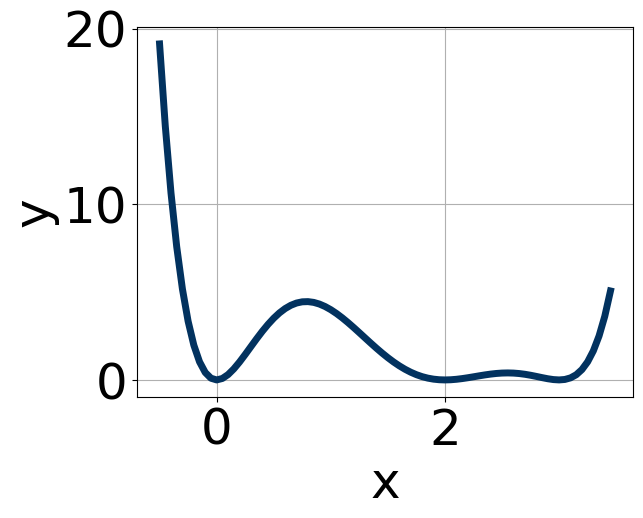
\includegraphics[width=0.5\textwidth]{../Figures/polyGraphToFunctionCopyB.png}
\end{center}


The solution is \( -5(x + 3)^{6} (x - 2)^{5} (x - 3)^{9} \), which is option E.\begin{enumerate}[label=\Alph*.]
\item \( 12(x + 3)^{8} (x - 2)^{11} (x - 3)^{9} \)

This corresponds to the leading coefficient being the opposite value than it should be.
\item \( -19(x + 3)^{6} (x - 2)^{10} (x - 3)^{11} \)

The factor $(x - 2)$ should have an odd power.
\item \( -20(x + 3)^{9} (x - 2)^{6} (x - 3)^{9} \)

The factor $-3$ should have an even power and the factor $2$ should have an odd power.
\item \( 6(x + 3)^{4} (x - 2)^{11} (x - 3)^{4} \)

The factor $(x - 3)$ should have an odd power and the leading coefficient should be the opposite sign.
\item \( -5(x + 3)^{6} (x - 2)^{5} (x - 3)^{9} \)

* This is the correct option.
\end{enumerate}

\textbf{General Comment:} General Comments: Draw the x-axis to determine which zeros are touching (and so have even multiplicity) or cross (and have odd multiplicity).
}
\end{enumerate}

\end{document}